%\documentclass{article}
\documentclass{chi2009}
\usepackage{times}
%\usepackage{uist}
\usepackage{url}
\usepackage{graphics}
\usepackage{color}

\newcommand{\want}[1]{{[\color{blue} WANT: #1]}}

\begin{document}

% --- Copyright notice ---
\conferenceinfo{UIST'09}{October 4-7, 2008, Victoria, BC, Canada}
\CopyrightYear{2009}
\crdata{x-xxxxx-xxx-x/xx/xxxx}

% Uncomment the following line to hide the copyright notice
\toappear{}
% ------------------------

\bibliographystyle{plain}

\title{Exposing Disputed Statements on the Web}

%%
%% Note on formatting authors at different institutions, as shown below:
%% Change width arg (currently 7cm) to parbox commands as needed to
%% accommodate widest lines, taking care not to overflow the 17.8cm line width.
%% Add or delete parboxes for additional authors at different institutions. 
%% If additional authors won't fit in one row, you can add a "\\"  at the
%% end of a parbox's closing "}" to have the next parbox start a new row.
%% Be sure NOT to put any blank lines between parbox commands!
%%

\author{
\parbox[t]{9cm}{\centering
	     {\em Author Name removed for blind review}\\
}
\parbox[t]{9cm}{\centering
	     {\em Author Name removed for blind review}}
}

\maketitle

%RULE: Don't cite media reports unless I have to

\abstract
We present DisagreeWeb, a browser extension that aims to let users see when the information they are reading presents only one side of a disputed issue. As the user browses the web, DisagreeWeb highlights snippets of text that make claims that conflict with information on other web sites. If a user clicks on such a disputed claim then DisagreeWeb will show tem an argument graph showing the best evidence for and against the claim being true, as determined by other users of DisagreeWeb.

\keywords{CSCW, sensemaking, web, browsers, collaboration, mind mapping} 

\classification{H5.2 [Information interfaces and presentation]:
User Interfaces. - Graphical user interfaces.}

\terms{Design, Human Factors}

\keywords{Sense-making, Annotation, Argumentation, Web}


\tolerance=400 
  % makes some lines with lots of white space, but 	
  % tends to prevent words from sticking out in the margin

\section{INTRODUCTION}

The web provides users with a huge number of pages that they can read, but extracting accurate and balanced information from these pages can be difficult. Not everything on the web is accurate~\cite{Mintz2002,Neumann2003,Resnik1998,Zhou2004} and many web sites have a strong political bias~\cite{Herman2002,Gentzkow2007}. If a user is to form a rounded opinion about a topic then they will need to either stick to sources that they trust or spend time looking for evidence on other web sites that supports or opposes what they read. Even if a user tries hard to research every topic they read, they can still get caught out by beliefs that they had not realised were disputed.

In this paper we present DisagreeWeb, a tool helps users discover when information they read is disputed or presents only one side of a contentious issue. When DisagreeWeb is used as a browser plugin it will highlight text that makes a disputed claim. If a user clicks on such a highlighted snippet then DisagreeWeb presents the user with an argument graph that shows the best evidence for and against the claim, as judged by other users of DisagreeWeb (Figure~\ref{claimview}). The argument graph contains links to snippets of text on other web sites that express conflicting or supporting points of view.

DisagreeWeb relies on users to identify disputed claims, to find appearances of these claims on web sites, and to vote for which snippets are most important.

\want{Seeded with all claims from Snopes}.
\want{Seeded with all contentious claims identified in the three months on FactCheck.org}
\want{Tested with hundreds of users}.
\want{Tested with real users and found took N seconds on average to identify and categorize snippets}

DisagreeWeb layers an argumentation graph over the existing web. 

\begin{figure}[tb]
	\begin{center}
	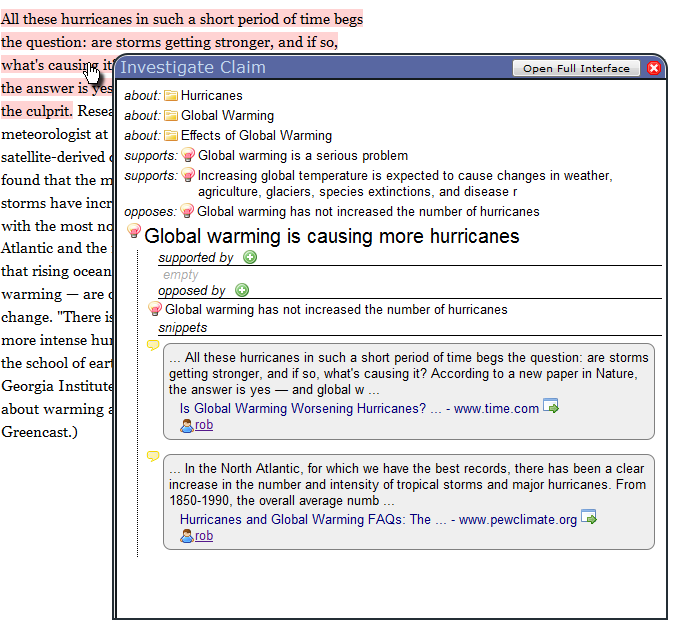
\includegraphics[width=6cm]{../screenshots/claim_popup_crop2.png}
	\caption{Click on a claim to investigate evidence for and against it}
	\label{claimview}
	\end{center}
\end{figure}

\section{RELATED WORK}


\section{HIGHLIGHTING CONTROVERSIAL CLAIMS}

\section{CONNECTING UP THE ARGUMENT}

\section{THE THINK LINK SYSTEM}

\section{USER STUDIES}

\section{CONCLUSIONS}

\bibliographystyle{abbrv}
\bibliography{refs}

\end{document}



